\documentclass{thureport}
% =============================================
% Part 1 Edit the info
% =============================================

\newcommand{\major}{软件71}
\newcommand{\name}{骆炳君}
\newcommand{\stuid}{2017013573}
\newcommand{\newdate}{2018-11-22}
\newcommand{\newtitle}{用传感器测空气相对压力系数}
\newcommand{\dL}{\delta L}
\def\celsius{{\ensuremath{^\circ\hspace{-0.09em}\mathrm{C}}}}

% =============================================
% Part 1 Main document
% =============================================
\begin{document}
\thispagestyle{empty}
\begin{figure}[h]
	\begin{minipage}{0.65\linewidth}
		\centerline{
\includegraphics[width=\linewidth]{head.jpg}}
	\end{minipage}
	\hfill
	\begin{minipage}{.3\linewidth}
		\raggedleft
		\begin{tabular*}{.8\linewidth}{ll}
			班级: & \underline\major   \\
			姓名: & \underline\name    \\
			学号: & \underline\stuid   \\
			日期: & \underline\newdate
		\end{tabular*}
	\end{minipage}
\end{figure}

\begin{table}[!htbp]
	\centering\large
	实验名称: \underline\newtitle
\end{table}

\tableofcontents
% =============================================
% Part 2 Main document
% =============================================
\newpage

\section{实验目的}
\begin{clause}
	\item 加深对理想气体状态方程和查理定律的理解.
	\item 初步了解铜电阻温度传感器和硅压阻式差压传感器的工作原理并掌握其作图方法.
	\item 学习用作图法和计算机作直线拟合法处理实验数据.
\end{clause}

\section{实验原理}
\subsection{理想气体的查理定律}
理想气体状态方程在定容条件下简化为查理定律
$$p=\frac{p_0T}{T_0}=p_0\frac{T_0+t}{T_0}=p_0(1+\alpha_pt)$$

其中为$\alpha_p$相对压力系数,定义为$\alpha_p=\frac{\Delta p}{p_0\Delta t}$,对于理想气体$\alpha_p=\frac{1}{T_0}=3.66\times10^{-3}\celsius^{-1}$,实际气体可近似看作理想气体.

根据查理定律可制作定容气体温度计,高准确度和灵敏度的定容温度计可用于检定其他类型的温度计.

\subsection{铜电阻温度传感器}
在范围内,铜丝的电阻值与温度有良好的线性关系
$$R=R_0(1+\alpha_Rt)$$

式中$\alpha_R$称为电阻温度系数.本实验中使用的铜丝电阻的$\alpha_R=4.26\times10^{-3}\celsius^{-1}$.

当铜丝电阻中通以恒定的电流$I$时
$$U_t=U_{R_0}(1+\alpha_Rt)$$

式中$U_{R_0}$为$0\celsius$时的电压,$U_{R_0}=IR_0$.

若测出了在纯水沸点时铜丝电阻的电压$U_{t_b}$和沸点$t_b$,有
$$t=\frac{U_t}{U_{t_b}}(\frac{1}{\alpha_R}+t_b)-\frac{1}{\alpha_R}$$

\subsection{扩散硅压阻式差压传感器}
当半导体材料因受力而产生应变时,由于载流子的浓度和迁移率的变化而导致电阻率发生变化的现象称为压阻效应.压阻式差压传感器的核心是硅膜片,这种膜片是利用制作集成电路的方法在单晶硅基片通过硼的扩散以形成如图1所示的十字形四段应变片.由于硅膜片是各向异性的,十字形四端应变片应设置在剪切应力最大的位置和剪切压阻系数最大的方向上.

\begin{figure}[h]
	\begin{minipage}[t]{0.4\linewidth}
		\centering
		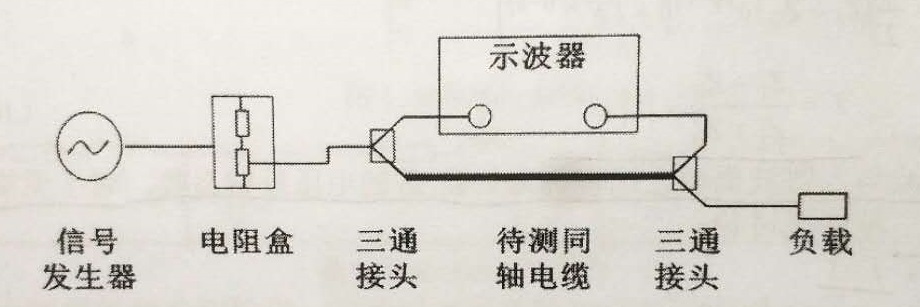
\includegraphics[height=3.5cm]{figure1.jpg}
		\caption{十字形四端应变片}
	\end{minipage}
	\hfill
	\begin{minipage}[t]{0.5\linewidth}
		\centering
		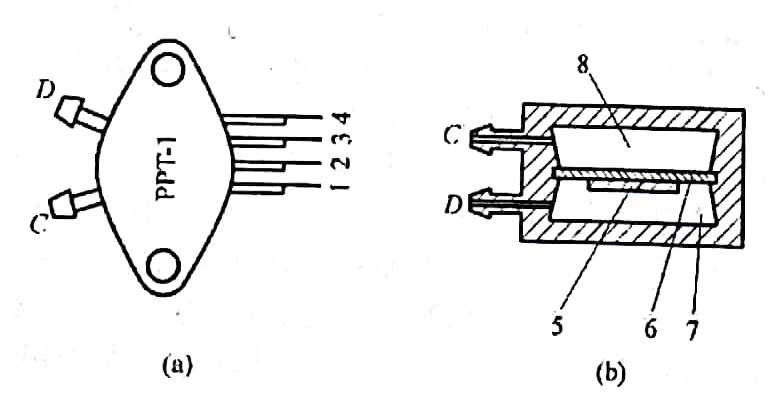
\includegraphics[height=3.5cm]{figure2.jpg}
		\caption{差压传感器结构示意图}
	\end{minipage}
\end{figure}

当膜片受应力时,若将一恒定电压E加在M和N两端上,在剪切应力作用下,从A和B两端会输出一与压值$\Delta p$成线性关系的电压$U_p$,且满足
$$U_p=U_0+k_p\Delta p$$

式中$U_0$为压差为0时的输出电压,系数$k_p$一般为常数.若传感器接口D通大气,接口C通被测介质,则
$$p=p_c+\frac{U_p-U_0}{k_p}$$

式中$p_c$为大气压强.该压阻式差压传感器的测量范围为$0\sim1.3\times10^5 Pa$,综合精度为$0.3\%$,它具有体积小,灵敏度高,稳定性好等优点.

\section{实验仪器}
\begin{figure}[h]
	\begin{minipage}[t]{0.45\linewidth}
		\centering
		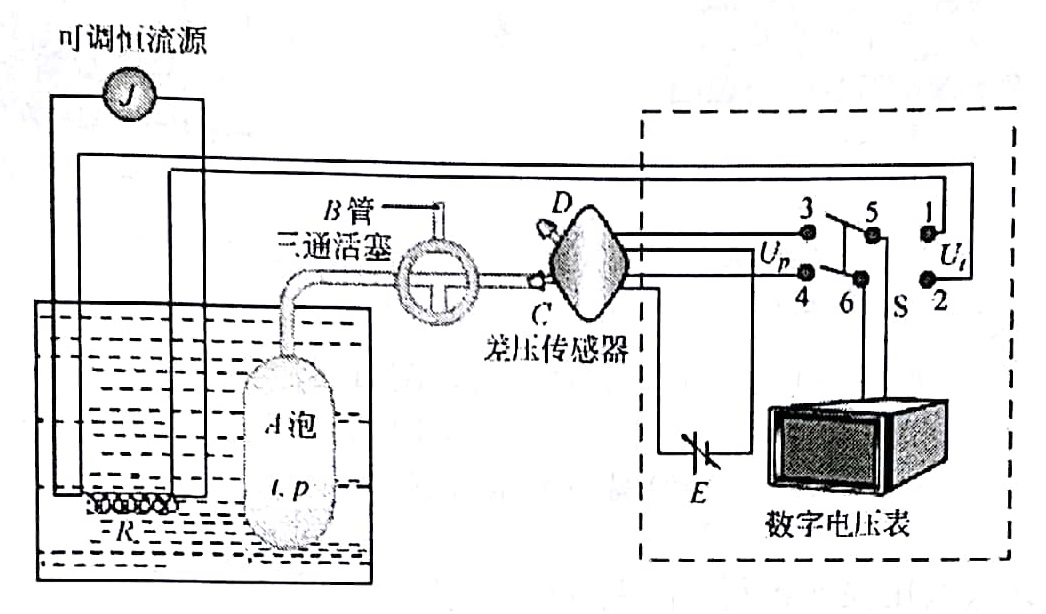
\includegraphics[height=4cm]{figure3.jpg}
		\caption{实验装置示意图}
	\end{minipage}
	\hfill
	\begin{minipage}[t]{0.45\linewidth}
		\centering
		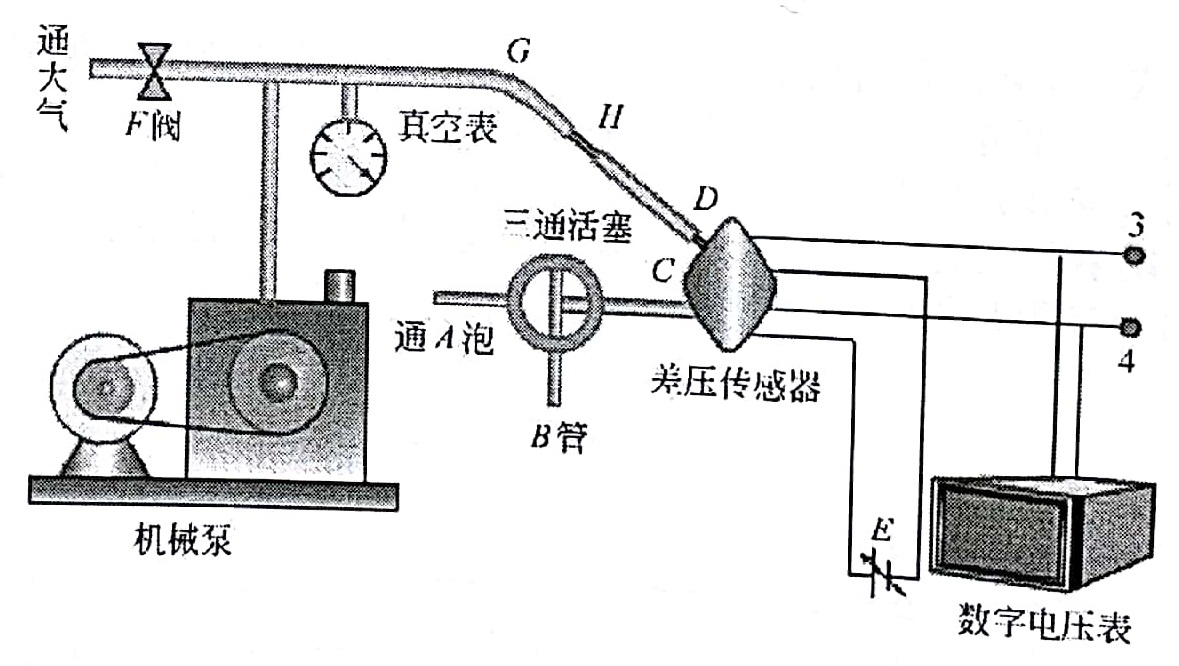
\includegraphics[height=4cm]{figure4.jpg}
		\caption{差压传感器定标装置示意图}
	\end{minipage}
\end{figure}

\section{实验步骤}
\subsection{差压传感器的定标}
用图4所示定标装置准确测定传感器的$U_0$和$k_p$.先转动三通管使传感器C口与B管相通,并使D口与机械泵相连,将四位半数字电压表接在差压传感器的输出端上,用泵从D口抽气,待电压表示数稳定(应最大)时,压差$\Delta p=p_c$,传感器输出电压记为$U_m$,然后停机械泵,使D口也通大气,此时$\Delta p=0$,电压表读数记为$U_0$,则
$$k_p=\frac{U_m-U_0}{p_c}$$

\subsection{测量若干组$(U_t,U_p)$值}
按图3接线,并使C口与A泡相通.调节恒流源J使电流约为$1.5\sim2.5mA$中的定值,记下室温下铜丝电压值$U_t$和传感器输出电压值$U_p$.加热,根据估计的铜丝电压间隔依次加热恒温后记录$(U_t,U_p)$值.最后记下水沸腾时的电压值,记为$(U_{t_b},U_{p_b})$.

实验前后用大气压强计各测一次大气压,同时记下室温值.

\subsection{实验注意事项}
\begin{clause}
	\item 加热时需用独立加热电源给加热器供电,用磁力搅拌器来搅拌,搅拌器转速应适当.
	\item “热得快”不能干烧,换水应先将加热电源断开,再将玻璃杯内的水倒入塑料桶.
	\item 小心操作以免损坏传感器和玻璃仪器.
	\item 停泵后应立即将机械泵抽气口通大气.
	\item 实验完毕将加热器的调速、温控旋钮调节至最小位置,并断开各电源开关.
\end{clause}

\section{数据处理}
\subsection{大气压强$p_c$与水的沸点值$t_b$}
实验前测得$p_c=101.66kPa$,查表有
$$p_{c1}=101.59kPa,\quad p_{c2}=101.72kPa$$
$$t_{b1}=100.07\celsius,\quad t_{b2}=100.11\celsius$$

由直线内插值法得
$$\frac{p_c-p_{c1}}{t_b-t_{b1}}=\frac{p_{c2}-p_{c1}}{t_{b2}-t_{b1}}$$

解得$t_b=100.09\celsius$

\subsection{差压传感器定标}
在C口通大气时测得$U_0=0.04mV$,在C口抽真空后测得$U_m=40.25mV$,得
$$k_p=\frac{U_m-U_0}{p_c}=0.3956mV/kPa$$

\subsection{$\Delta U_t$的估算}
初始时,测得室温$t=19.8\celsius$,$U_t=126.32mV$

要使得从室温到$80\celsius$能够测得11组数据,取$\Delta t=6\celsius$

有$$U_{R_0}=\frac{U_t}{1+\alpha_Rt}=116.49mV$$

所以$$\Delta U_t=U_{R_0}\alpha_R\Delta t=2.98mV$$

\subsection{$U_t$、$U_p$数据的处理}

实验测得数据见下表

\begin{table}[H]
	\centering
	  \begin{tabular}{|c|c|c|c|}
	  \hline
	  $U_t/mV$ & $t/\celsius$     & $U_p/mV$ & $p/Pa$ \bigstrut\\
	  \hline
	  126.47  & 20.19  & 0.04  & $1.0166\times10^5$ \bigstrut\\
	  \hline
	  129.45  & 26.19  & 0.18  & $1.0201\times10^5$ \bigstrut\\
	  \hline
	  132.54  & 32.42  & 1.26  & $1.0474\times10^5$ \bigstrut\\
	  \hline
	  135.36  & 38.11  & 2.16  & $1.0702\times10^5$ \bigstrut\\
	  \hline
	  138.08  & 43.59  & 2.80  & $1.0864\times10^5$ \bigstrut\\
	  \hline
	  141.26  & 50.00  & 3.73  & $1.1099\times10^5$ \bigstrut\\
	  \hline
	  144.51  & 56.55  & 4.69  & $1.1341\times10^5$ \bigstrut\\
	  \hline
	  147.61  & 62.80  & 5.51  & $1.1549\times10^5$ \bigstrut\\
	  \hline
	  $166.11\ (U_{t_b})$  & $100.09\ (t_b)$  & $10.22\ (U_{p_b})$  & $1.2739\times10^5\ (p_b)$ \bigstrut\\
	  \hline
	  \end{tabular}%
\end{table}%

其中
$$t=\frac{U_t}{U_{t_b}}(\frac{1}{\alpha_R+t_b})-\frac{1}{\alpha_R}$$
$$p=p_c+\frac{U_p-U_0}{k_p}$$

实验时用计算机进行直线拟合得(见附图5)
$$p=(93803+339.89t)Pa,\quad r=0.999$$
$${\alpha_p}_0=\frac{339.89}{93803}=3.6234\times10^{-3}\ (\celsius^{-1})$$

根据经验公式修正
$$\delta \alpha_p=(0.018+5\frac{v}{V})\times10^{-3}=0.118\times10^{-3}\ (\celsius^{-1})$$

所以最终结果为
$$\alpha_p={\alpha_p}_0+\delta \alpha_p=3.7414\times10^{-3}\ \celsius^{-1}$$

在坐标纸上通过作图法得(见附图6)
$$p=(94.0+0.33333t)kPa$$

$${\alpha_p}_0=\frac{0.33333}{94.0}=3.5461\times10^{-3}\ (\celsius^{-1})$$

根据经验公式修正
$$\delta \alpha_p=(0.018+5\frac{v}{V})\times10^{-3}=0.118\times10^{-3}\ (\celsius^{-1})$$

所以最终结果为
$$\alpha_p={\alpha_p}_0+\delta \alpha_p=3.6641\times10^{-3}\ \celsius^{-1}$$

和计算机拟合直线基本吻合.

\section{实验结果}
本实验利用铜电阻温度传感器和硅压阻式差压传感器,采取水浴加热的方法测量空气(可近似为理想气体)在定容条件下的多组压强、温度数据,并进行直线拟合,在误差允许的范围内验证了理想气体查理定律,测得了空气相对压力系数,取得了较好的实验结果.

\section{思考题}
\subsection*{1.}
应先转动三通活塞使传感器C口与B管连通而与A断开,同时C通大气,然后用机械泵从D口抽气,电压表读数达最大并稳定后记为$U_m$,然后停泵,并使D口也通大气,此时电压表读数即为$U_0$,由$k_p=\frac{U_m-U_0}{p_c}$便可得到$k_p$.

若D口漏气,则用机械泵抽气后$\Delta p<p_c$,$U_m$偏小,故$k_p$偏小.

\subsection*{2.}
热平衡时电压表示数稳定,读数才准确.若不控制热平衡,装置内可能有局部温差,导致读数不准.

若升温过快,热量来不及扩散而聚集在局部,会导致读出的$U_t$和$U_p$不准确,而且示数会随着热量的扩散而不断变化,不易读数.

\subsection*{3.}
三通活塞属玻璃制品易损坏,转动时应缓慢,并用另一只手扶住活塞外壳.

换水要先将加热器电源断开,再将玻璃系统拿下放在备用的空烧杯上,把水浴杯内的水直接倒入热水回收桶,注意搅拌子别倒掉.

\subsection*{4.}
可能是由于仪器漏气.因为沸腾时A泡与大气压差较大,三通活塞很可能漏气,从而使A泡内气体减少,气压下降,从而导致$U_p$单调下降.

\clearpage
\section{拟合曲线}
\begin{figure}[h]
	\centering
	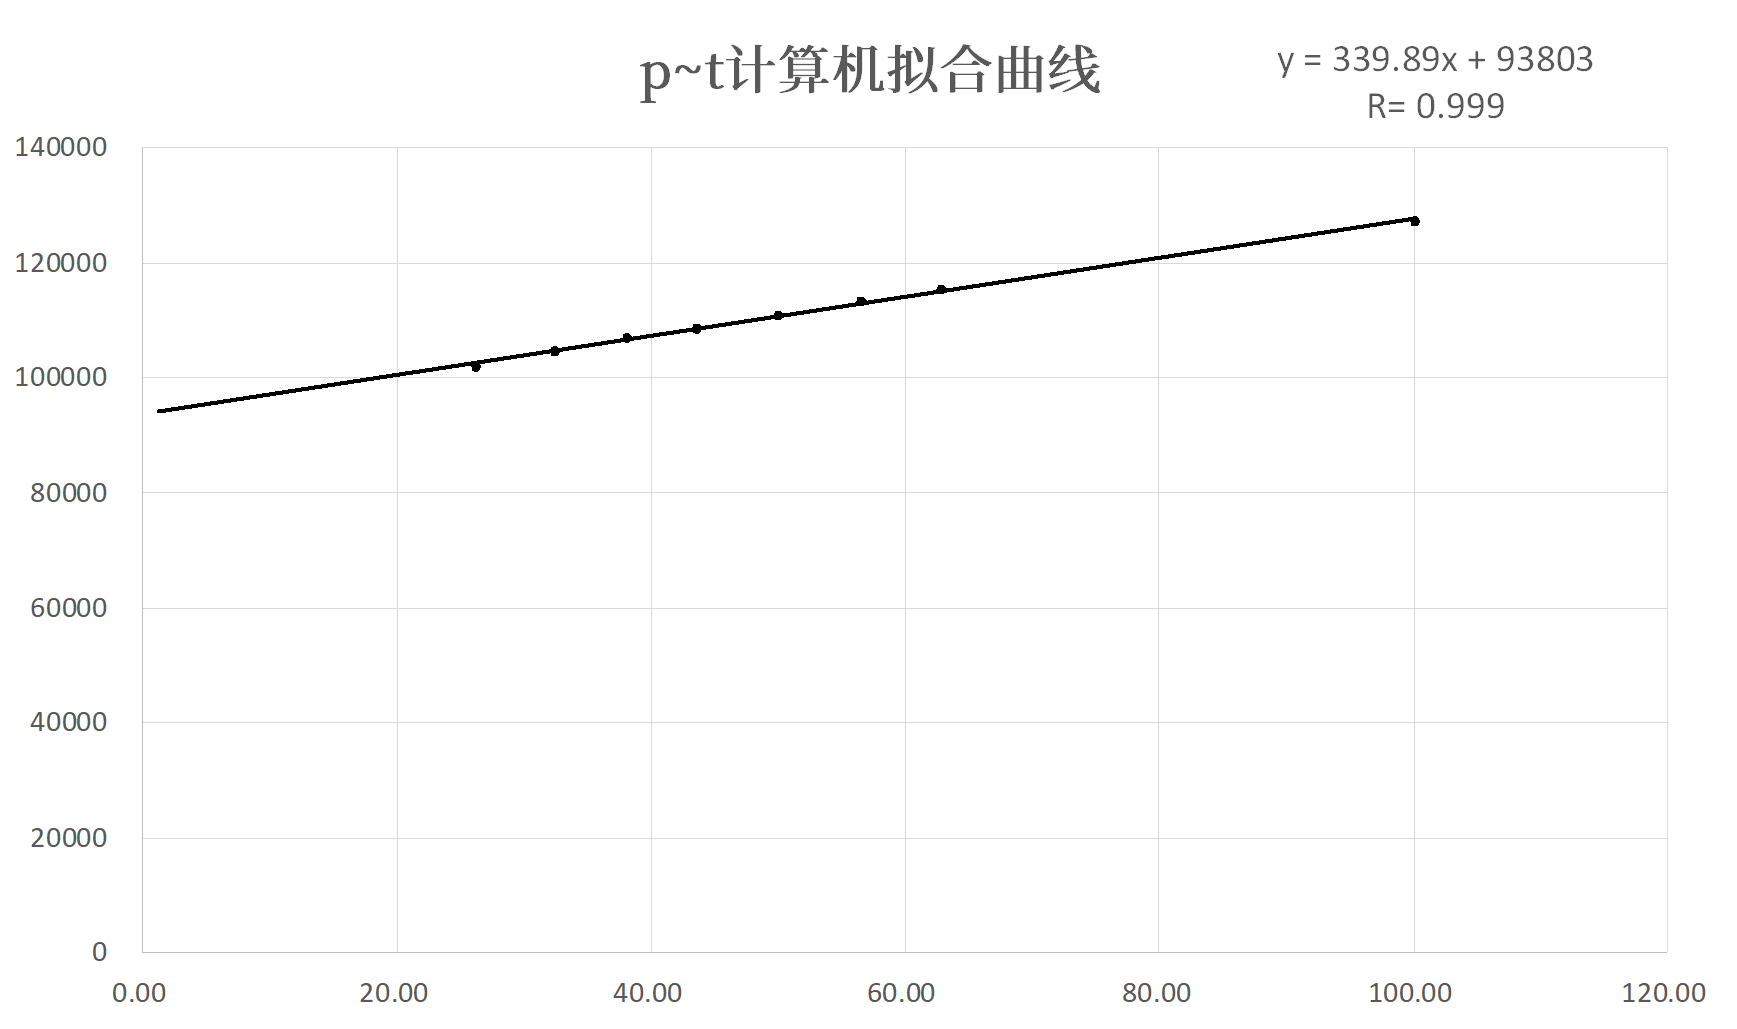
\includegraphics[width=0.9\linewidth]{figure3.png}
\end{figure}

\begin{figure}[h]
	\centering
	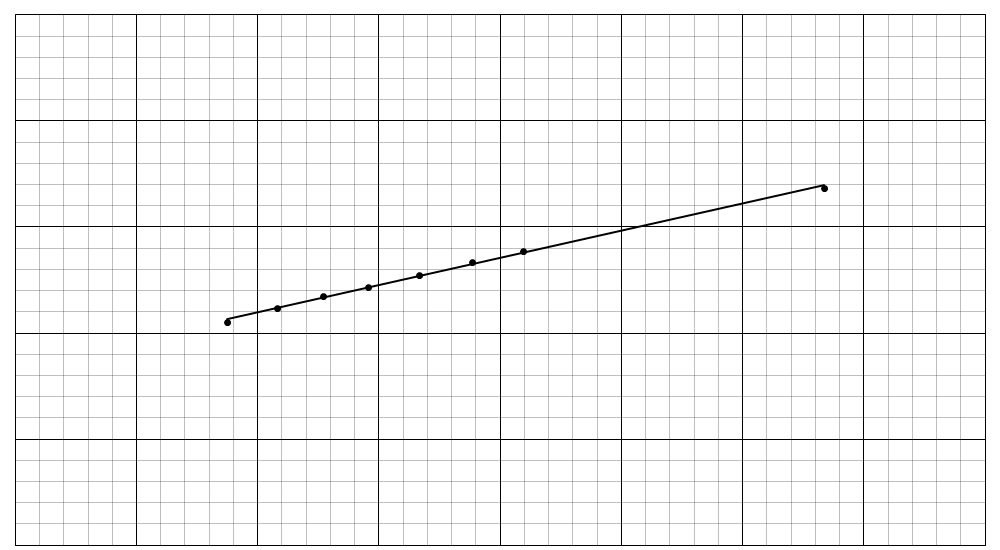
\includegraphics[width=0.9\linewidth]{figure4.png}
\end{figure}

\newpage
\section{原始数据表格}

\end{document}